%+----------------------------------------------------------------------------+
%| SLIDES: 
%|
%| Contents:	- 60 minutes, hybrid format (handwritten + overlays)
%|
%| Author: Antonio miti
%| Place: Higher Geometry Seminars, Bonn
%| Date: 15/12/21
%+----------------------------------------------------------------------------+



%- D0cum3nt ----------------------------------------------------------------------------------------------
\documentclass[10pt]{beamer}



%- Packages -------------------------------------------------------------------------------------------
\usepackage{custom-style}
\usepackage{multicol}
\usepackage{stmaryrd}
\usepackage{animate}
\usetikzlibrary{positioning, arrows}
\usetikzlibrary{shapes}
\usepackage{fontawesome}



%--Beamer Style----------------------------------------------------------------------------------------
\usetheme{toninus}
\setbeamertemplate{section in toc}[sections numbered]



%-- Macros ----------------------------------------------------------------------------------------

\providecommand{\pairing}{\langle\cdot,\cdot\rangle}
\providecommand{\vHam}{\mathscr{v}}
\renewcommand{\checkpoint}[0]{
	\setcounter{tocdepth}{1}
	\addtocounter{framenumber}{-1}
 	\begin{frame}[t]{Outline}
  		%\tableofcontents[currentsection,currentsubsection]
  		%
  		\tableofcontents[currentsection]
		%
		\begin{center}
			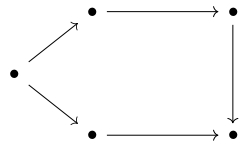
\includegraphics[width=3.5cm]{Pictures/Figure_pentagondiagm_page}
		\end{center}
	\end{frame}
}



%- T1tle P4g3 -------------------------------------------------------------------------------------------
\title{
Multisymplectic observables and higher Courant algebroids
}
\subtitle{\href{https://arxiv.org/abs/2209.05836}{arXiv:2209.05836} (j.w. Marco Zambon)}
\author[AMM]{\href{https://dmf.unicatt.it/miti/}{Antonio Michele Miti}}
\institute[UCSC]{
  \begin{tabular}[h]{ccc}
      &Università Cattolica del Sacro Cuore& \\
      &Brescia, Italy& \\
      &\href{https://dipartimenti.unicatt.it/dmf-home?rdeLocaleAttr=it}{
\includegraphics[width=3.5cm]{Logos/UnicattBS-logo}} &
  \end{tabular}      
}
\date[Template_21] % (optional, should be abbreviation of conference name)
{	
	{\vskip 2ex}
	\href{https://www.mathematik.uni-wuerzburg.de/mathematicalphysics/forschung/veranstaltungen/workshops-und-konferenzen/single/news/poisson-geometry-higher-structures-and-deformation-theory/}{Poisson Geometry, Higher Structures, and Deformation Theory} \\
	{\vskip 1ex}
	Würzburg, September 21, 2023
}







%---------------------------------------------------------------------------------------------------------------------------------------------------
%- D0cum3nt ----------------------------------------------------------------------------------------------------------------------------------
\begin{document}
%-------------------------------------------------------------------------------------------------------------------------------------------------

	\titlepage


%-------------------------------------------------------------------------------------------------------------------------------------------------
\iffalse \section{Introduction}\fi
%-------------------------------------------------------------------------------------------------------------------------------------------------


%-------------------------------------------------------------------------------------------------------------------------------------------------
\begin{frame}[t] % Hybrid format - Title Page
	%
	\begin{center}
	\color{UniGreen}
		\par\noindent\rule{\textwidth}{0.4pt}\\[.5em]	
		{\bf\Large\emph{Multisymplectic observables }}
		\\
		and 
		{\bf\Large\emph{higher Courant algebroids}}\\
		\par\noindent\rule{\textwidth}{0.4pt}			
	\end{center}
	\vfill

	\centering
	\begin{tikzpicture}
		\node [draw,ellipse callout,UniGreen, minimum height=16em,minimum width=33em,callout relative pointer={(0,1)}] (L1) {};
		\node [text width=28em,text centered] (L2) {
			\textcolor{UniGreen}{\textbf{Honest Goals} of the talk:}
			\\
			\medskip
			\begin{itemize}[<+->]
				\item[•] Recall a certain "gauge-compatibility" condition in \emph{symplectic} geometry 
				   \color{blue}\small (involving $\omega$-twisted Lie alg.oids)
				\item[•] Discuss how this condition extends to \emph{\textbf{multi}symplectic} geometry
				   \color{blue}\small (involving $\omega$-twisted higher Courant alg.oids)
				\item[•] Review certain multisymplectic constructions guided by the above problem.\\
			\end{itemize}
			\medskip
		};
	\end{tikzpicture}

\end{frame}
\addtocounter{framenumber}{-1}
%-------------------------------------------------------------------------------------------------------------------------------------------------


%%-------------------------------------------------------------------------------------------------------------------------------------------------
%\begin{frame}[fragile]{A \emph{pentagonal} diagram in symplectic geometry}
%	Given a \alert{symplectic mfd.} $(M,\omega)$ ...
%	\vfill
%	\begin{center}
%		\includestandalone[width=.95\textwidth]{Pictures/Frame_Embedding_Diagram_symplectic}
%	\end{center}
%	\vspace{3em}
%	\vfill
%	\begin{minipage}[t][8.5em][t]{\textwidth}
%		\begin{itemize}
%			\item<1-> \alert<1>{... there is a naturally associated Poisson algebra ...}
%			\item<2-> \alert<2>{... and also a (standard twisted) Lie Algebroid}.
%			\item<3-> A Lie algebroid is a "controlled" \alert<3>{$\infty$-dimensional Lie algebra.}
%			\item[]<4->
%				\quad\\
%		\vspace{-.75em}
%		\tcbset{colback=white,
%		colbacktitle=white,
%		colframe=red!70!black,
%		boxrule=1pt,
%		colupper=red!70!black,
%		arc=15pt,
%		}
%		\begin{tcolorbox}[enhanced,frame hidden,borderline={0.5pt}{0pt}{blue}]
%			\color{blue}{
%			\textbf{Lemma}: There exists an embedding of Lie Algebras.
%			}
%		\end{tcolorbox}
%		\end{itemize}
%	\end{minipage}
%\end{frame}
%%-------------------------------------------------------------------------------------------------------------------------------------------------

%-------------------------------------------------------------------------------------------------------------------------------------------------
\begin{frame}[fragile]{A \emph{pentagonal} diagram in symplectic geometry}
	Given a \alert{symplectic mfd.} $(M,\omega)$ ...
	\vfill
	\begin{center}
		\includestandalone[width=.95\textwidth]{Pictures/Frame_Embedding_Diagram_symplectic}
	\end{center}
	\vfill
	\begin{minipage}[t][8.5em][t]{\textwidth}
		\begin{itemize}
			\only<1-3>{
			\item<1-> \alert<1>{... there is a naturally associated Poisson algebra ...}
			\item<2-> \alert<2>{... and also a (standard twisted) Lie Algebroid}.
			\item<3-> A Lie algebroid is a "controlled" $\infty$-dimensional Lie algebra given (in this case) by
			\begin{displaymath}
					\left[\binom{x_1}{f_1},\binom{x_2}{f_2}\right]
					~=~
					\binom{[x_1,x_2]}{x_1(f_2)-x_2(f_1)-\omega(x_1,x_2)}
				\end{displaymath}
			}
			\item[]<4->
				\quad\\
				\begin{thmblock}[There exists an embedding of Lie algebras.]
					\begin{displaymath}
						\begin{tikzcd}
							\Psi~:&[-1em] C^{\infty}(M)_\omega \ar[r,"\Psi"]& \Gamma(TM\oplus \mathbb{R})_\omega
							\\[-2em]
							& f \ar[r,mapsto] & \binom{\mathscr{v}_f}{f}
						\end{tikzcd}		
					\end{displaymath}
				\end{thmblock}
		\end{itemize}
	\end{minipage}
\end{frame}
\note{}
%-------------------------------------------------------------------------------------------------------------------------------------------------


%-------------------------------------------------------------------------------------------------------------------------------------------------
\begin{frame}[fragile]{A \emph{pentagonal} diagram in symplectic geometry}
	%
Consider two \alert{gauge-related} symplectic mfd. $(M,\omega)$ and $ (M,\widetilde{\omega})$.
	%
	\begin{center}
			\includestandalone[width=.8\textwidth]{Pictures/hyb-Frame_BigDiagram_symplectic}
	\end{center}
		\vfill
	\begin{minipage}[t][8em][t]{\textwidth}
		\begin{itemize}
			\only<3-4>{
				\item<3-> There is a natural \alert<3>{isomorphism in the Lie Alg.oids category} \emph{($B$-transformation)}
					\begin{displaymath}
						\binom{x}{f} \mapsto \binom{x}{f-\iota_x B} ~.
					\end{displaymath}~.
				\item<4-> It descends to an \alert<4>{isomorphism of Lie algebras}.
			}
			\only<6-8>{
				\item<6-> \vspace{-2em}Consider an infinitesimal \alert<6>{Hamiltonian group action} $\mathfrak{g}\circlearrowleft M$ w.r.t. both $\omega$ and $\tilde{\omega}$.
				\item<7-> let be $f:\mathfrak{g} \to C^\infty(M)_\omega$ and $\tilde{f}:\mathfrak{g} \to C^\infty(M)_{\tilde{\omega}}$ two comoment map s.t.
				\begin{displaymath}
					\tilde{f}(\xi) = f(\xi) - \iota_{\underline{\xi}}B
				\end{displaymath}
				}
			\item[]						
		\end{itemize}
	\only<2>{
		\vspace{-.75em}
		\begin{center}
		\tcbox[enhanced,frame hidden,borderline={0.5pt}{0pt}{red,dashed}]{	
			\alert{
			\faQuestionCircle \qquad
				{How can we compare the two \emph{observables} algebras?}
			\qquad \faQuestionCircle		
			}
		}
		\end{center}
	}
	\only<5>{
		\vspace{-.75em}
		\begin{center}
		\tcbox[enhanced,frame hidden,borderline={0.5pt}{0pt}{red,dashed}]{	
			\alert{
			\faQuestionCircle \qquad
				{How can we close the left-hand side?}
			\qquad \faQuestionCircle		
			}
		}
		\end{center}
	}
	\only<8->{
		\vspace{-.75em}
		\tcbset{colback=white,
		colbacktitle=white,
		colframe=red!70!black,
		boxrule=1pt,
		colupper=red!70!black,
		arc=15pt,
		}
		\begin{tcolorbox}[enhanced,frame hidden,borderline={0.5pt}{0pt}{blue}]
			\color{blue}{
			\textbf{Lemma}: The central pentagon commutes!
			}
		\end{tcolorbox}
	\vfill
	}
	\end{minipage}	
\end{frame}
%-------------------------------------------------------------------------------------------------------------------------------------------------


%%-------------------------------------------------------------------------------------------------------------------------------------------------
%\begin{frame}[fragile]{Compatibility between gauge transformations and comoment maps}
%	%
%	Consider $(M,\omega)$ \alert{symplectic mfd.}
%	%
%	\begin{center}
%			\includestandalone[width=.8\textwidth]{Pictures/Frame_BigDiagram_symplectic}
%	\end{center}
%	%
%	\vspace{-1em}
%	\vfill
%	\begin{minipage}[t][8em][t]{\textwidth}
%		\begin{itemize}
%			\only<2>{
%				\item<2-> Consider a second gauge-related symplectic structure on $M$
%					\begin{displaymath}
%						\tilde{\omega} = \omega + d B \qquad \text{with} \quad B\in \Omega^1(M).
%					\end{displaymath}
%			}
%			\only<3-4>{
%				\item<3-> There is a natural isomorphism in the Lie Alg.oids category \emph{($B$-transformation)}
%					\begin{displaymath}
%						\binom{x}{f} \mapsto \binom{x}{f-\iota_x B} ~.
%					\end{displaymath}
%			}
%			\only<6-7>{
%				\item<6-> Consider an infinitesimal group action $\mathfrak{g}\circlearrowleft M$ which is Hamiltonian w.r.t. both $\omega$ and $\tilde{\omega}$.
%				\item<7-> let be $f:\mathfrak{g} \to C^\infty(M)_\omega$ and $\tilde{f}:\mathfrak{g} \to C^\infty(M)_{\tilde{\omega}}$ two comoment map s.t.
%				\begin{displaymath}
%					\tilde{f}(\xi) = f(\xi) - \iota_{\underline{\xi}}B
%				\end{displaymath}
%				}
%			\item[]						
%		\end{itemize}
%	\only<5>{
%		\vspace{-.75em}
%		\begin{center}
%		\tcbox[enhanced,frame hidden,borderline={0.5pt}{0pt}{red,dashed}]{	
%			\alert{
%			\faQuestionCircle \qquad
%				{How can we close the left-hand side?}
%			\qquad \faQuestionCircle		
%			}
%		}
%		\end{center}
%	}
%	\only<8->{
%		\vspace{-.75em}
%		\tcbset{colback=white,
%		colbacktitle=white,
%		colframe=red!70!black,
%		boxrule=1pt,
%		colupper=red!70!black,
%		arc=15pt,
%		}
%		\begin{tcolorbox}[enhanced,frame hidden,borderline={0.5pt}{0pt}{blue}]
%			\color{blue}{
%			Lemma: The central pentagon commutes!
%			}
%		\end{tcolorbox}
%	\vfill
%	}
%	\only<9->{
%		\vspace{-.75em}
%		\begin{center}
%		\tcbox[enhanced,frame hidden,borderline={0.5pt}{0pt}{red,dashed}]{	
%			\alert{
%			\faQuestionCircle \qquad
%				{What happens in the higher (n-plectic) case?}
%			\qquad \faQuestionCircle		
%			}
%		}
%		\end{center}
%	}
%	\end{minipage}	
%\end{frame}
%\note[itemize]{
%	\item The horizontal embedding is  $f \mapsto (v_f,f)$;
%	\item Vertical maps are also known as \emph{Gauge transformations}
%	\item upshot: 
%	\begin{enumerate}
%		\item 
%	\end{enumerate}
%}
%%-------------------------------------------------------------------------------------------------------------------------------------------------





%-------------------------------------------------------------------------------------------------------------------------------------------------
\begin{frame}[fragile]{A \emph{pentagonal} diagram in symplectic geometry}
	%
Consider two \alert{gauge-related} symplectic mfd. $(M,\omega)$ and $ (M,\widetilde{\omega})$.
	%
	\begin{center}
			\includestandalone[width=.8\textwidth]{Pictures/hyb-image_BigDiagram_symplectic}
	\end{center}
	%
	\vfill
	\begin{minipage}[t][8em][t]{\textwidth}
	\centering
	\vspace{-2em}
	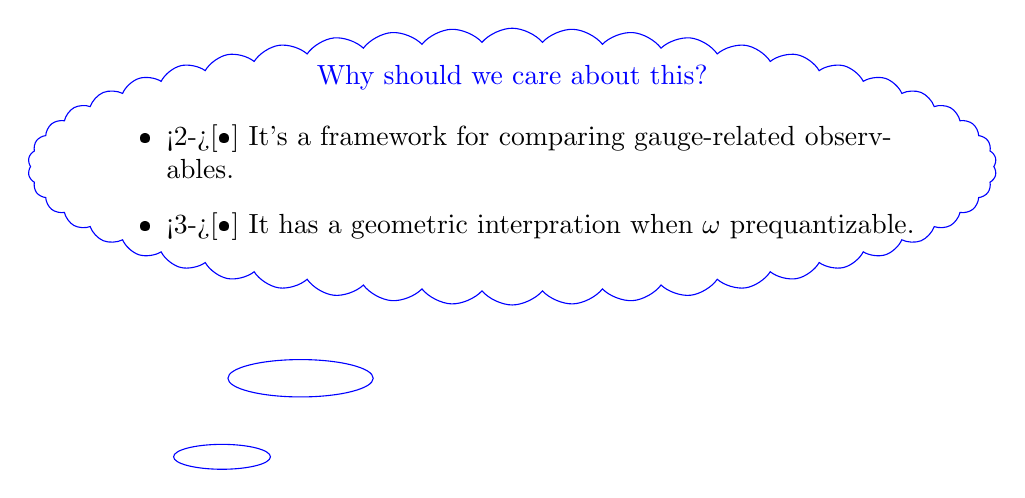
\begin{tikzpicture}
		\node [draw,cloud callout,cloud puffs=50,cloud puff arc=100,blue, minimum height=10em,minimum width=35em,callout relative pointer={(-2,-2)}] (L1) {};
		\node [text width=30em,text centered] (L2) {
			\textcolor{blue}{Why should we care about this?}
			\\
			\begin{itemize}
				\item<2->[•] It's a framework for comparing gauge-related observables.
				\item<3->[•] It has a geometric interpration when $\omega$ \alert{prequantizable}.
			\end{itemize}
			\medskip
		};
	\end{tikzpicture}
	\end{minipage}	
\end{frame}
%-------------------------------------------------------------------------------------------------------------------------------------------------



%-------------------------------------------------------------------------------------------------------------------------------------------------
\begin{frame}[t]{Scope of the talk}
		\begin{center}
		\tcbox[enhanced,frame hidden,borderline={0.5pt}{0pt}{red,dashed}]{	
			\alert{
			\faQuestionCircle \qquad
				{\bf  What happens in the (higher) $n$-plectic case?}
			\qquad \faQuestionCircle		
			}
		}
		\end{center}
		\vfill

	\only<2->{
		{
			\color{UniGreen}
			\par\noindent\rule{\textwidth}{0.4pt}	
			\\ {\bf  Outline of the talk:} \\[-.5em]
			\par\noindent\rule{\textwidth}{0.4pt}			
		}
		\vspace{-1.5em}
		\setcounter{tocdepth}{1}
		\tableofcontents
	}
\end{frame}
%-------------------------------------------------------------------------------------------------------------------------------------------------







%-------------------------------------------------------------------------------------------------------------------------------------------------
\section{What is \textbf{multisymplectic geometry}?}
\checkpoint	
%-------------------------------------------------------------------------------------------------------------------------------------------------


\begin{frame}[t, fragile]{Multisymplectic manifolds} %Fragile -->workaround tikzcd
	\begin{center}
		$-$ \emph{multisymplectic means \textbf{going higher} in the degree of $\omega$} $-$
	\end{center}
	\pause
	\begin{defblock}[$n$-plectic manifold ~\emph{(Cantrijn, Ibort, De Le\'on)} \cite{Cantrun2017}]
		\includestandalone[width=0.95\textwidth]{Pictures/hyb-Figure_multisym}	
	\end{defblock}
	%
	\vfill
	%
	%
	\pause
	\begin{block}{Examples:}
		\begin{itemize}
			\item[$\bullet$] 1-plectic $=$ symplectic
			\item[$\bullet$] Any oriented $(n+1)$-dimensional manifold is $n$-plectic w.r.t. the volume form.
			\item[$\bullet$] The multicotangent bundle $\Lambda^n T^\ast Q$ is naturally $n$-plectic.
		\end{itemize}
	\end{block}			 
%
	\pause
	\begin{block}{Historical motivation}
		Mechanics: geometrical foundations of \textit{(first-order)} field theories.
		\begin{itemize}
		 \item[•] Kijowski, W. Tulczyjew \cite{Kijowski1979}; %(1979)
		 \item[•] Cariñena, Crampin, Ibort \cite{Carinena1991b};% (1991)
		 \item[•] Gotay, Isenberg, Marsden, Montgomery \cite{Gimmsy1};%(1998)
		 \\ $\cdots$
		\end{itemize}
	\end{block}
\end{frame}


%-------------------------------------------------------------------------------------------------------------------------------------------------
\section{What is the \textbf{higher analogue} of the \textbf{Poisson algebra}?}
\checkpoint	
%-------------------------------------------------------------------------------------------------------------------------------------------------


\begin{frame}{Hamiltonian forms}
	\only<1>{
	\medskip
	\begin{columns}[T]
		\setlength{\belowdisplayskip}{5pt}
		\begin{column}{.50\linewidth}
			\centering \it
			$-$ symplectic case $-$
			\vspace{20em}		
		\end{column}	
		%
		\onslide{\vrule{}}
		%
		\begin{column}{.50\linewidth}
			\centering \it
			$-$ $n$-plectic case $-$
			\vspace{20em}		
		\end{column}	
	\end{columns}
	}
	\pause
	%
	\begin{defblock}[Hamiltonian $(n-1)$-forms]
		\begin{displaymath}
			\Omega^{n-1}_{ham}(M,\omega) 	:=
			\biggr\{ \sigma \in  \Omega^{n-1}(M) \; \biggr\vert \; 
				\exists \vHam_\sigma \in \mathfrak{X}(M) ~:~ 
				\tikz[baseline,remember picture]{\node[rounded corners,
                        fill=orange!5,draw=orange!30,anchor=base]            
            			(target) {$d \sigma = -\iota_{\vHam_\sigma} \omega$ };
            	}				
				~\biggr\} 
			\end{displaymath}
	\end{defblock}
	%
	\onslide<2>{
		\tikz[overlay,remember picture]
		{
			\node[rounded corners,
                 fill=orange!5,draw=orange!30,anchor=base]
            	 (base) at ($(current page.north east)-(2,1)$) [rotate=-0,text width=3.5cm,align=center] {\footnotesize{\textcolor{red}{Hamilton-DeDonder-Weyl \\equation}}};
		}	
		\begin{tikzpicture}[overlay,remember picture]
		    	\path[->] (base.south east) edge[bend left,red](target.east);
	    \end{tikzpicture}
	}
	%
	\vspace{-1em}
	\begin{columns}[T]
		\setlength{\belowdisplayskip}{5pt}
		\begin{column}{.50\linewidth}
			%
			\centering \it
			$-$ symplectic case $-$
			\onslide<3->{
			\begin{thmblock}[Observables Poisson algebra]
				$C^\infty(M,\omega)$ endowed with
				\vspace{-.5em}
				\begin{displaymath}
					\lbrace \sigma_1, \sigma_2 \rbrace =			
					~ - \iota_{\vHam_1}\iota_{\vHam_2} \omega 
					~= \mathcal{L}_{\vHam_1} \sigma_2
				\end{displaymath}			
				forms a Poisson algebra.
			\end{thmblock}
			}
			%
			\onslide<4->{
			\vspace{1em}
			\begin{itemize}
				\item[\cmark] Skew-symmetric;
				\item[\cmark] multiplication of observables;
				\item[\cmark] Leibniz Rule;
				\item[\cmark] Jacobi equation;
			\end{itemize}		
			}		
		\end{column}	
		%
		\onslide<1->{\vrule{}}
		%
		\begin{column}{.50\linewidth}
			\centering \it
			$-$ $n$-plectic case $-$
			\onslide<5->{			
			\begin{thmblock}[Observables $L_\infty$-algebra]
				$\Omega^{n-1}_{ham}(M,\omega)$ endowed with
				\vspace{-.5em}
				\begin{displaymath}
					\lbrace \sigma_1, \sigma_2 \rbrace =			
					~ - \iota_{\vHam_1}\iota_{\vHam_2} \omega 
				\end{displaymath}			
				can be extended to a \\ $L_\infty-algebra$.
			\end{thmblock}
			}
			%
			\onslide<6->{
			\begin{itemize}
				\item[\cmark] Skew-symmetric;
				\item[\xmark] multiplication of observables;
				\item[\xmark] Jacobi equation;
				%\\ \hspace*{4.25em} full-fledged Jacobi equation;
				\item[\smark] Jacobi equation \emph{up to homotopies}.
			\end{itemize}			
			}
		\end{column}	
	\end{columns}
\end{frame}
%-------------------------------------------------------------------------------------------------------------------------------------------------

%------------------------------------------------------------------------------------------------
\begin{frame}{Reminder: $L_\infty$ Algebras}

		\emph{
			$L_\infty$-algebra is the notion that one obtains from a Lie algebra when one requires the Jacobi identity to be satisfied only up to a higher coherent chain homotopy.
		}
		\\
		\vspace{.5em}
		\begin{defblock}[$L_\infty$-algebra ~\emph{(Lada, Markl)} ~\cite{Lada1995}]
			\includestandalone{Pictures/Figure_Linfinitydef}
		\end{defblock}	
		%
		%
	\pause
%	\vfill
%	\begin{thmblock}[Rogers \cite{Rogers2010}]
%		The \emph{higher observable algebra} $L_{\infty}(M,\omega)$ 	forms an honest $L_\infty$ algebra.
%		\footnotetext{ Take $\mu_1 = \text{d}$, $\mu_k=\lbrace\dots\rbrace_k$, $L$ is a shifted truncation of the de Rham complex.}
%	\end{thmblock}

	\begin{itemize}
		\item<2-> You can construct a coalgebra out of $L$ 
			{\small \color{UniGreen} (the reduced cofree coalgebra $S^{\geq 1}(L[1]),\Delta)$)}.
		\item<3-> You can assemble all $\mu_k$ to get a coderivation $Q_\mu$
				{\small \color{UniGreen} (the unique lift to a coderivation of the decalage of $ \mu=	\mu_1+\mu_2 + \dots$ }.
		\item<4-> Higher Jacobi is tantamount to having $Q_\mu ^2 = 0$.

	\end{itemize}
\end{frame}
\note[itemize]{
	\item $L_\infty$-algebra is the notion obtained from a Lie algebra requiring that the Jacobi identity is satisfied only up to a higher coherent chain homotopy.
	\item The Lie-n algebra mentioned before is a $L_\infty$ algebra with underlying graded vector space concentrated in degrees $0,1...n$.
	
	\item Definition. We say that a permutation $\sigma \in S_n$ is a $(j,n-j)$-unshuffle, $0\leq j \le1 n$  if $\sigma(1)< \dots < \sigma(j)$ and $\sigma(j+1)<\dots<\sigma(n)$.
	\\
	You can also say that $\sigma$ is a $(j,n-j)$-unshuffle if $\sigma(i)< \sigma(i+1)$ when $i\neq j$.

	\item 	Alternatively, the Jacobiators can be also denoted as $$\displaystyle J_m=\sum_{i+j=m+1} 	\mu_i \triangleleft \mu_j = 0$$
	employing the so-called \emph{ Richardson-Nijenhuis product}
		 $$\mu_i\circ \mu_j := (-)^{i(j+1)}\frac{1}{j!(i-1)!}\mu_i \triangleleft \mu_j\otimes \mathbb{1}_{i-1} \circ \mathcal{A}~,$$
		 where $\mathcal{A}$ denotes the (graded) total skew-symmetrizator.
		 
	\item see frame extra-\ref{Frame:unwapping-Jacobi} for a slightly demystification of the higher Jacobi equations.

	\item more precisely this statement is a proposition/definition

}
%------------------------------------------------------------------------------------------------


%-------------------------------------------------------------------------------------------------------------------------------------------------
\begin{frame}[fragile]{Lie $\infty$-algebra of Observables (higher observables) }
	Let be $(M,\omega)$ a $n$-plectic manifold.
	  	\vfill
	\begin{defblock}[$L_\infty$-algebra of observables ~\emph{(Rogers)} \cite{Rogers2010}]
		\medskip
		\hspace{.25em} Is a cochain-complex $(L,\{\cdot\}_1)$ \\
		\vspace{-1em}
		\begin{center}
			\includestandalone{Pictures/hyb-Frame_Observables}
		\end{center}
		\onslide<2->{
			\bigskip
			\hspace{.25em} with $n$ (skew-symmetric) multibrackets $(2 \leq k \leq n+1)$\\
			\vspace{-1em}
			\onslide<3->{
				\begin{center}
					\includestandalone{Pictures/Equation_Multibracket}	
				\end{center}
			}
			\medskip
		}
		%
	\end{defblock}
%	\onslide<3->{
%		\emph{Higher analogue} of the \emph{Poisson algebra structure} associated to a symplectic mfd.
%	\vfill
%	\begin{columns}
%		\hfill
%		\begin{column}{.11\linewidth}	
%			If $n>1$:
%			
%		\end{column}	
%		\begin{column}{.8\linewidth}
%		\begin{itemize}
%			\item[\xmark] \textcolor{red}{we lose} :\quad multiplication of observables, Jacobi equation;
%			%\\ \hspace*{4.25em} full-fledged Jacobi equation;
%			\item[\cmark] \textcolor{green}{we gain} :\quad brackets with arities different than two,\\
%			\hspace*{4.25em}
%			 Jacobi equation \emph{up to homotopies}.
%		\end{itemize}		
%		\end{column}		
%	\end{columns}
%	}
  \end{frame}
%-------------------------------------------------------------------------------------------------------------------------------------------------


%-------------------------------------------------------------------------------------------------------------------------------------------------
\section{What is the \textbf{higher analogue} of the \textbf{twisted Lie algebroid}?}
\checkpoint	
%-------------------------------------------------------------------------------------------------------------------------------------------------

%-------------------------------------------------------------------------------------------------------------------------------------------------
\begin{frame}[t]{Vinogradov Algebroids}
	\begin{defblock}[Vinogradov algebroid (higher Courant)]
		\includestandalone[width=0.95\textwidth]{Pictures/hyb-Frame_vinogradov}		
	\end{defblock}
	\vfill
	\begin{itemize}
		\item<7-> $(n=1) ~ \Rightarrow$ standard twisted \emph{Lie algebroid};
		\item<8-> $(n=2) ~ \Rightarrow$ standard twisted \emph{Courant algebroid};
	\end{itemize}

\end{frame}
%-------------------------------------------------------------------------------------------------------------------------------------------------


%-------------------------------------------------------------------------------------------------------------------------------------------------
\begin{frame}[fragile]{Vinogradov $L_\infty$-algebra}
	Vin. alg.oids 
	$\quad\simeq\quad$ 	
	$NQ$-manifolds {\small($L_\infty$-algebroids)}
	$\quad\Rightarrow\quad$ 
	{\small Associated} $L_\infty$-algebra
	%
	\pause
	\begin{defblock}[Vinogradov $L_\infty$-algebra (Zambon) \cite{Zambon2012}]
		\includestandalone[width=0.95\textwidth]{Pictures/hyb-Frame_vinogradov-Linfty}	
	\end{defblock}
	\vfill
	\only<5->{
		\tikz[overlay,remember picture]
		{
			\node[rounded corners,
                 fill=gray!1,draw=gray!30,anchor=base]            
            	 (base) at ($(current page.south)+(0,.5)$) [rotate=-0,text width=10cm,align=center] { \footnotesize{\color{gray}{
            	 $e_i = \binom{X_i}{\alpha_i} \in \mathfrak{X}(M)\oplus \Omega^{n-1}(M)$ 
            	 \quad~,\qquad
            	 $f_i \in \bigoplus_{k=0}^{n-2}\Omega^k(M)$.
            	 }}};
		}			
	}

\end{frame}
%-------------------------------------------------------------------------------------------------------------------------------------------------












%-------------------------------------------------------------------------------------------------------------------------------------------------
\section{What is the \textbf{higher analogue} of the \textbf{comoment map}?}
\checkpoint	
%-------------------------------------------------------------------------------------------------------------------------------------------------

%-------------------------------------------------------------------------------------------------------------------------------------------------
\begin{frame}[t]{Comoment maps}
	Consider a Lie algebra action $v:\mathfrak{g} \to \mathfrak{X}(M)$  preserving the $n$-plectic form $\omega$,
	\vfill

	\vspace{-1em}
	\begin{columns}[T]
		\setlength{\belowdisplayskip}{5pt}
		\begin{column}{.50\linewidth}
			%
			\centering \it
			\onslide<2->{
				$-$ symplectic case $-$
				\begin{defblock}[Comoment map pertaining to $v$]
					Lie algebra morphism
					$$ f: \mathfrak{g} \to C^\infty(M) $$
					such that
					$$ d~f (x) = -\iota_{v_x} \omega \qquad \forall x \in \mathfrak{g}~.$$
				\end{defblock}
			}
		\end{column}	
		%
		\onslide<2->{\vrule{}}
		%
		\begin{column}{.50\linewidth}
			\centering \it
			\onslide<3->{			
				$-$ $n$-plectic case $-$
				\begin{defblock}[Homotopy comoment map \tiny (HCMM)]
					$L_\infty$-morphism 
					$$ (f_k) : \mathfrak{g} \to L_\infty (M,\omega)$$
					such that
					$$ d~f_1(x) = -\iota_{v_x} \omega \qquad \forall x \in \mathfrak{g}~.$$
				\end{defblock}	
			}
		\end{column}	
	\end{columns}	
	%
	\pause
	\vfill
	\centering 
	\onslide<4->{\textbf{-- Conserved quantities --}}
	%
	\vspace{-1em}
	\begin{columns}[T]
		\setlength{\belowdisplayskip}{5pt}
		\begin{column}{.50\linewidth}
			%
			\centering \it
			\onslide<4->{
			\begin{propblock}[Noether Theorem]
				\small Fixed $H\in C^\infty_{\text{Ham}}(M)$ ($\mathfrak{g}$-invariant) ,
				$$\mathcal{L}_{v_H} f(x) = 0 \qquad \forall x \in \mathfrak{g}$$
			\end{propblock}
			}
		\end{column}	
		%
		\onslide<5->{\vrule{}}
		%
		\begin{column}{.50\linewidth}
			\centering \it
			\onslide<5->{			
			\begin{propblock}[RWZ16 Theorem]
				\small Fixed $H\in \Omega^{n-1}_{\text{Ham}}(M)$ ($\mathfrak{g}$-invariant),
				$$\mathcal{L}_{v_H} f_k(p) \in B^k(M) \qquad \forall p \in Z_k(\mathfrak{g})$$			
			\end{propblock}
			}
		\end{column}	
	\end{columns}		
\end{frame}
%-------------------------------------------------------------------------------------------------------------------------------------------------




%-------------------------------------------------------------------------------------------------------------------------------------------------
\begin{frame}{Gauge related multisymplectic manifolds and comoment maps}
	Consider $M$ smooth mfd.
	%
	\begin{defblock}[Gauge related $n$-plectic structures]
		\bigskip
		\begin{columns}[T]
			\setlength{\belowdisplayskip}{5pt}
			\begin{column}{.50\linewidth}
				%
				\centering \it
				\onslide<2->{
				$\quad\omega,~ \tilde{\omega}~ \in \Omega^{n+1}(M)$ multisymplectic,
				}
			\end{column}	
			%
			\begin{column}{.50\linewidth}
				\centering \it
				\onslide<3->{			
				such that $\omega = \tilde{\omega} - d B$
				}
			\end{column}	
		\end{columns}	
		\bigskip	
	\end{defblock}
	%
	\pause
	\vfill
	\par\noindent\rule{\textwidth}{0.4pt}	
	\vfill
	\pause
	%
	Consider \quad $v:\mathfrak{g} \to \mathfrak{X}(M)$ preserving $\omega$ and $\tilde{\omega}$,
	%\phantom{consider}\quad $\mathcal{L}_{v_\xi}\omega=\mathcal{L}_{v_\xi}\tilde{\omega} = 0 \quad \forall \xi \in \mathfrak{g}$
	\\
	let \qquad$f: \mathfrak{g}\to L_\infty(M,\omega)$ an \emph{homotopy comoment map} ~ w.r.t. $\mathfrak{g}\circlearrowleft (M,\omega)$
	\pause
	\begin{lemblock}[Also $(M,\tilde{\omega})$ admits HCMM $(\tilde{f})$]
		\medskip
		\begin{columns}
			\begin{column}{.325\linewidth}
					\onslide<5->{
						\begin{displaymath}
							\tilde{f}_k = f_k +	
								\tikz[baseline,remember picture]{\node[rounded corners,
	                        		fill=blue!5,draw=blue!30,anchor=base]            
	            					(target) {$\mathrm{b}_k$ };
	            					}	
						\end{displaymath}
					}		
			\end{column}
			\begin{column}{.625\linewidth}	
					\onslide<5->{
						\begin{displaymath}
						%
						\begin{tikzcd}[baseline=(O.base),ampersand replacement=\&]
							|[alias=O]| 
							\tikz[baseline,remember picture]{\node[rounded corners,
	                        		fill=blue!2,draw=blue!30,align=center]            
	            					(base) {$\mathrm{b}_k$};}						
							~:\&[-3em] \Lambda^k\mathfrak{g} \ar[r]\& \Omega^{n-k}(M)
							\\[-2em]
							\& \xi_1\wedge\dots \xi_k \ar[r,mapsto] \&
							(-)^k \iota(v_{\xi_1})\dots \iota(v_{\xi_{x_k}}) B
						\end{tikzcd}		
						\end{displaymath}								
					}		
			\end{column}
		\end{columns}
		\bigskip
		\only<5->{
			\begin{tikzpicture}[overlay,remember picture]
			    	\path[->,opacity=0.3] (base.west) edge[bend left,blue](target.south east);
		    \end{tikzpicture}		
	    }
	\end{lemblock}
	%
\end{frame}
%-------------------------------------------------------------------------------------------------------------------------------------------------


%-------------------------------------------------------------------------------------------------------------------------------------------------
\section{What is the \textbf{higher pentagonal diagram}?}
\checkpoint	
%-------------------------------------------------------------------------------------------------------------------------------------------------

%-------------------------------------------------------------------------------------------------------------------------------------------------
\begin{frame}{Checkpoint}
	We ends up with the following diagram \onslide<2->{\emph{in the $L_\infty$-algebras category}}
	\vfill
	%
	\only<2->{\vspace{-2em}}
	\begin{center}
		\includestandalone[width=.9\textwidth]{Pictures/hyb-Frame_Diagram_checkpoint}
	\end{center}	
	\vfill
	\vspace{-2em}
	\onslide\onslide<2->{Open questions:}
	\begin{itemize}
		\item<3->[-] Does {\color{blue!60!black}\textbf{Rogers} $L_\infty$ \textbf{embeds} into \textbf{Vinogradov}}?
		\item<4->[-] Are {\color{green!60!black} \textbf{gauge related Vinogradov} $L_\infty$-algebras \textbf{isomorphic}}?
		\item<5->[-] Does the {\color{red!60!black} pentagonal \textbf{diagram commute}}?
	\end{itemize}


\end{frame}
%-------------------------------------------------------------------------------------------------------------------------------------------------


%-------------------------------------------------------------------------------------------------------------------------------------------------
\subsection{Does Rogers $L_\infty$ embeds into Vinogradov?}
\subcheckpoint	
%-------------------------------------------------------------------------------------------------------------------------------------------------
%-------------------------------------------------------------------------------------------------------------------------------------------------
\begin{frame}[fragile,t]{Embedding observables $L_\infty$-algebra into Vinogradov $L_\infty$-algebra}
	Consider now $\omega$ \alert{$n$-plectic}~.
	\vfill
	\only<4->{\vspace{-5em}}
	\begin{center}
		\includestandalone[width=.8\textwidth]{Pictures/hyb-Frame_Embedding_Diagram_k-plectic}
	\end{center}
	\vfill
	\begin{minipage}[t][8.5em][t]{\textwidth}
	\only<4->{
	\begin{thmblock}[Embedding of $L_\infty$-algebras  $\Psi:L_\infty(M,\omega)\hookrightarrow L_{\infty}(E^n,\omega)$\quad \cite{Miti2022}.]
	\begin{itemize}[leftmargin=0pt]
		\item[$\cdot$]<5-> 
			consider the graded vector subspace $\mathcal{A}$
			\onslide<6->{
				\begin{displaymath}
				\mathclap{
				{\mathcal{A}^k} =
				\begin{cases}
			\left.\left\lbrace
			\binom{X}{\alpha}\in \mathfrak{X}(M)\oplus \Omega^{n-1}(M)
			~ \right\vert ~
			\iota_X \omega = -d \alpha\right\rbrace
	&\quad k=0,\\
					\Omega^{n-1+k}(M) &\quad -n+1 \leq k < 0.
				\end{cases}			
				}
				\end{displaymath}	
			}					
		\item[$\cdot$]<6-> 
			restrict the two $L_\infty$-structures to $\pi$ and $\mu$ on $\mathcal{A}$
		\item[$\cdot$]<7->

			$L_\infty(M,\omega) \cong 
				(\mathcal{A},\pi) \color{red}\cong\color{black}
				(\mathcal{A},\mu) \hookrightarrow
				L_\infty(E^n,\omega)$
	\end{itemize}
	\end{thmblock}
	}
	\end{minipage}
\end{frame}
%-------------------------------------------------------------------------------------------------------------------------------------------------



%-------------------------------------------------------------------------------------------------------------------------------------------------
\subsection{Are gauge related Vinogradov $L_\infty$-algebras isomorphic?}
\subcheckpoint	
%-------------------------------------------------------------------------------------------------------------------------------------------------

%-------------------------------------------------------------------------------------------------------------------------------------------------
\begin{frame}[t]{Higher $B$-transformation}
	Consider now $\omega$ \alert{n-plectic} \quad and \quad \alert{$\tilde{\omega}=\omega + d B$}:
		\medskip
	\only<4->{\vspace{-2em}}			
	\begin{center}
		\includestandalone[width=.4\textwidth]{Pictures/hyb-Frame_multisym_B-transf}
	\end{center}
	\vfill
	\only<1>{
	\begin{itemize}
		\item Vinogradov alg.oids w.r.t cohomologous twisting closed forms are isomorphic.
		\\
		\small{(in a suitable sense)}
	\end{itemize}	
	}
	%	
	\onslide<3->{
		\vspace{-1em}
		\begin{thmblock}[There is a \textbf{strict} $L_\infty$-isomorphism.]	
				\begin{displaymath}
				%
				\only<3>{
				\begin{tikzcd}[baseline=(O.base),ampersand replacement=\&]
					|[alias=O]| 
					(\varphi)				
					~:\&[-3em] L_\infty(E^n,\omega) \ar[r,"\sim"]\& L_\infty(E^n,\tilde{\omega})
				\end{tikzcd}	
				\vspace{3.5em}
				}
				\only<4->{
				\begin{tikzcd}[baseline=(O.base),ampersand replacement=\&]
					|[alias=O]| 
					(\varphi)				
					~:\&[-3em] L_\infty(E^n,\omega) \ar[r,"\sim"]\& L_\infty(E^n,\tilde{\omega})
					\\[-1em]
					\varphi_1				
					~:\&[-3em] \left(\mathcal{V}^n\right)_0 \ar[r,"\sim"] \& (\widetilde{\mathcal{V}}^n)_0=\mathfrak{X}(M)\oplus\Omega^{n-1}(M)
					\\[-2em]
					\& \binom{x}{\alpha} \ar[r,mapsto] \&
					\binom{x}{\alpha +\iota_x B}
				\end{tikzcd}	
				}
				\end{displaymath}
			\vspace{-1em}		
		\end{thmblock}							
	}		
\end{frame}
%-------------------------------------------------------------------------------------------------------------------------------------------------




%-------------------------------------------------------------------------------------------------------------------------------------------------
\subsection{Does the pentagonal \textbf{diagram commute}?}
\subcheckpoint	
%-------------------------------------------------------------------------------------------------------------------------------------------------


%-------------------------------------------------------------------------------------------------------------------------------------------------
\begin{frame}{The higher pentagonal diagram}
	Consider now $\omega$ \alert{n-plectic} \quad and \quad \alert{$\tilde{\omega}=\omega + d B$}:
	\vfill
	%
	\only<2->{\vspace{-2em}}
	\begin{center}
		\includestandalone[width=.8\textwidth]{Pictures/hyb-Frame_Gauge_Diagram_k-plectic}
	\end{center}	
	%
	\only<2->{\vspace{-2em}}
	%
	\vfill
	%
	\begin{itemize}
		\item<2-> Vinogradov $L_\infty$-algebras w.r.t cohomologous twisting forms are isomorphic.
		\item<2-> Rogers $L_\infty$ embeds into Vinogradov $L_\infty$.
		\item<3-> Consider a Lie algebra action $\mathfrak{g}\to \mathfrak{X}(M)$ admitting HCMM w.r.t $\omega$ and $\tilde{\omega}$
	\end{itemize}

	\vfill
	\tcbset{colback=white,
		colbacktitle=white,
		colframe=blue!70!black,
		boxrule=1pt,
		colupper=blue!70!black,
		arc=15pt,
		}
	\onslide<4->{
	\begin{tcolorbox}[sidebyside,righthand width=.75\linewidth]
		Thm: \cite{Miti2022}
		\tcblower
		\color{blue}
The pentagon commutes. 
			\\\emph{(On the nose, not "up to homotopies")}.
	\end{tcolorbox}	
	
	}
	

\end{frame}
%-------------------------------------------------------------------------------------------------------------------------------------------------



	\begin{frame}{}
	\label{frame:thankyouslide}
		\vfill
	  \centering 
	  {\Huge\color{red} 
	  \emph{Thank you for your attention!}}
		\vfill
		%
		\centering
		\fbox{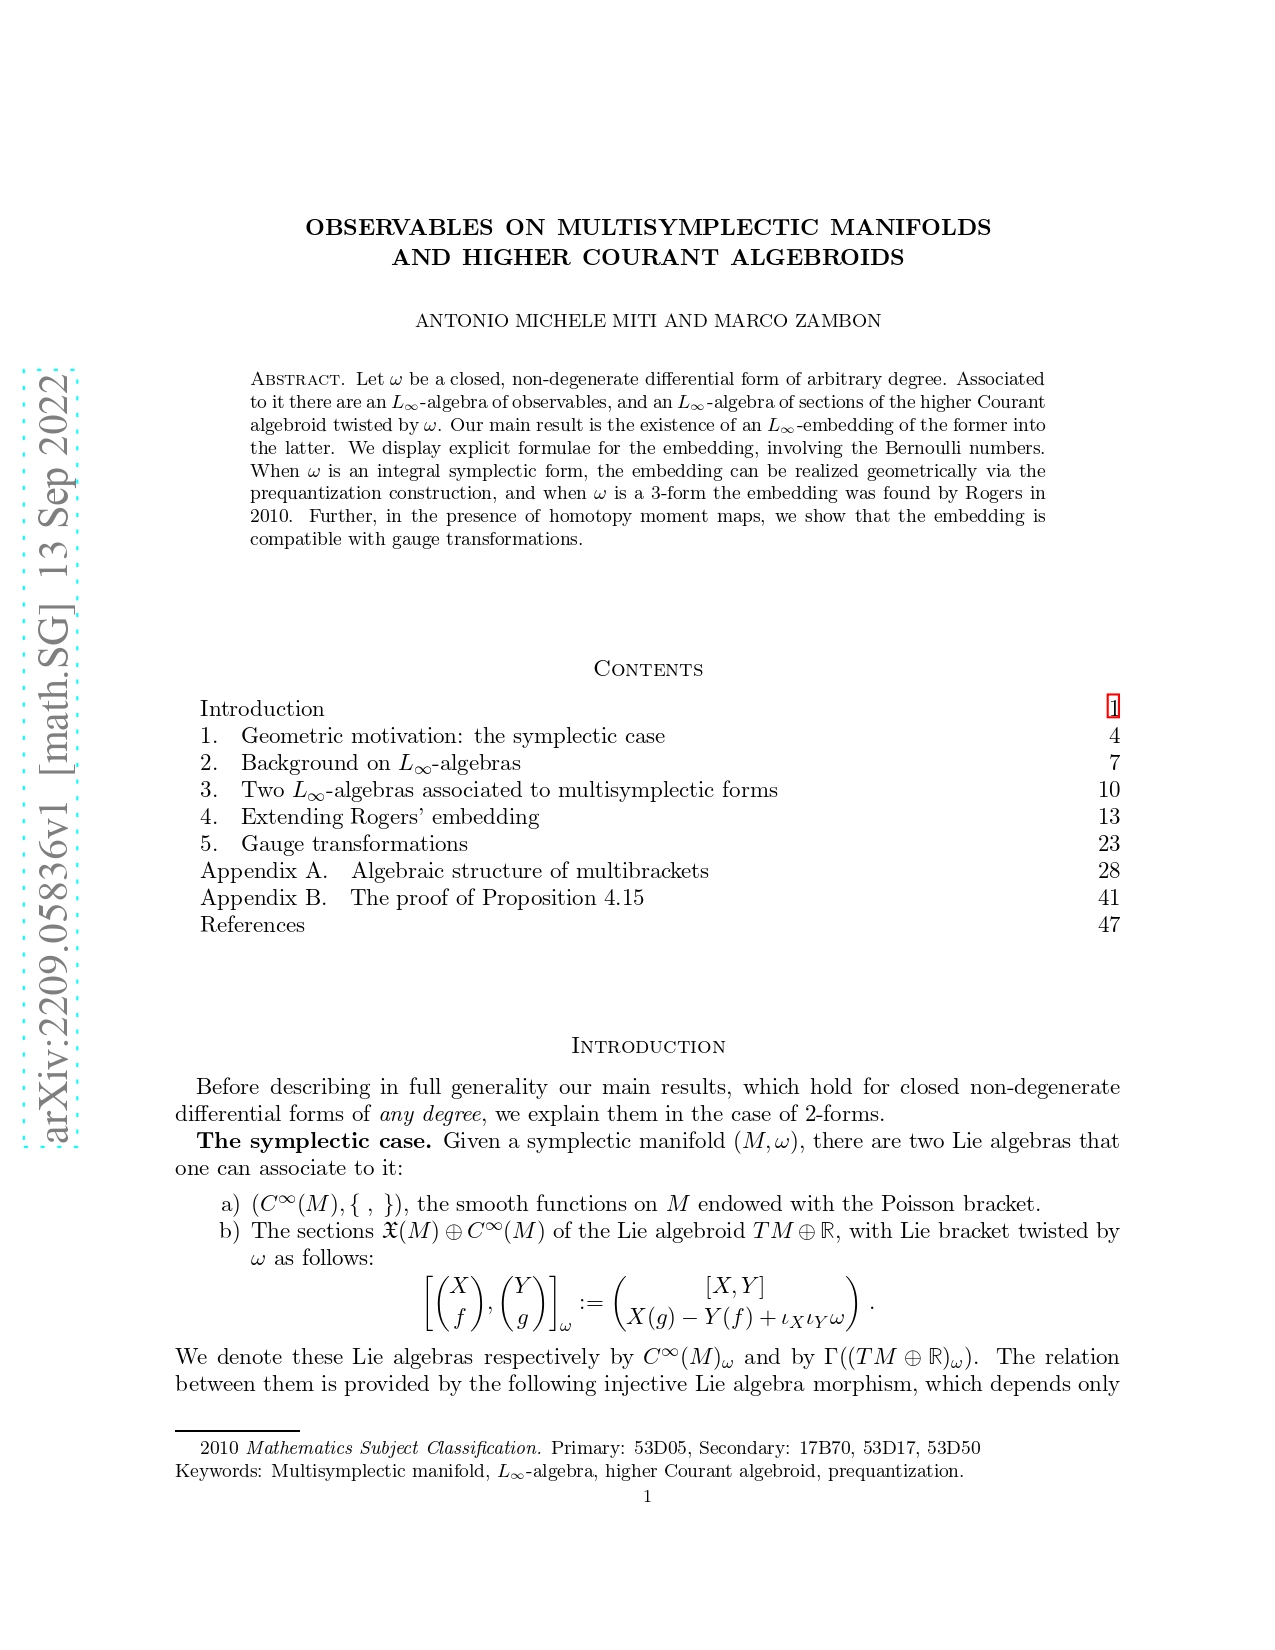
\includegraphics[width=.4\textwidth]{Pictures/arxiv-cover}}
	\end{frame}




%------------------------------------------------------------------------------------------------
% APPENDIX
%------------------------------------------------------------------------------------------------
\appendix



%-------------------------------------------------------------------------------------------------------------------------------------------------
\section{Appendix}
%------------------------------------------------------------------------------------------------

%-------------------------------------------------------------------------------------------------------------------------------------------------
\begin{frame}[fragile]{Homotopy comomentum maps}
	Consider a Lie algebra action $v:\mathfrak{g} \to \mathfrak{X}(M)$  \underline{preserving the $n$-plectic form $\omega$}.
	\vfill
	\begin{defblock}[Homotopy comomentum map \emph{(Callies, Fregier, Rogers, Zambon)} \cite{Callies2016}]
			\includestandalone{Pictures/Frame_Lifting}
	\end{defblock}
	\onslide<4->{
	\begin{lemblock}[HCMM unfolded  \cite{Callies2016}]
			%
			HCMM is a sequence of (graded-skew) multilinear maps:
			\begin{displaymath}
				(f)  = \big\lbrace f_k: \; \Lambda^k{\mathfrak g} \to L^{1-k} \subseteq \Omega^{n-k}(M) 
				~\big\vert~ 0\leq k \leq n+1  \big\rbrace
			\end{displaymath}
			\emph{fulfilling:}%\emph{such that:}
			\begin{itemize}
				\item<5-> $f_0 = 0 $, $f_{n+1} = 0$
				\item<6-> $d f_k (p) = f_{k-1} (
				\tikz[baseline,remember picture]{\node[rounded corners,
                        fill=green!5,draw=green!30,anchor=base]            
            			(target) {$\partial $ };
            	}				
				p)  - (-1)^{\frac{k(k+1)}{2}} \iota(v_p) \omega 
				\qquad\scriptstyle \forall p \in \Lambda^k(\mathfrak{g}),\; \forall k=1,\dots n+1$
			\end{itemize}
		\onslide<7->{
			\tikz[overlay,remember picture]
			{
				\node[rounded corners,
	                 draw=green!30,anchor=base]            
	            	 (base) at ($(current page.east)-(3,3)$) [rotate=-0,align=center] {\footnotesize{\hyperlink{frame:CE-complex}{\emph{Chevalley-Eilenberg boundary op.}}}};
			}	
		\begin{tikzpicture}[overlay,remember picture]
	    	\path[->] (base.west) edge[bend right,green](target.north east);
	    \end{tikzpicture}
	    }
	\end{lemblock}	
	}
	\vfill
\end{frame}
%-------------------------------------------------------------------------------------------------------------------------------------------------



%------------------------------------------------------------------------------------------------
% https://en.wikibooks.org/wiki/LaTeX/Bibliographies_with_biblatex_and_biber
\begin{frame}[t,allowframebreaks]{Extended Bibliography}
	\bibliographystyle{alpha}
	\bibliography{bibfile}
\end{frame}
%------------------------------------------------------------------------------------------------









%------------------------------------------------------------------------------------------------
\end{document}

